\PassOptionsToPackage{unicode=true}{hyperref} % options for packages loaded elsewhere
\PassOptionsToPackage{hyphens}{url}
%
\documentclass[
  ignorenonframetext,
]{beamer}
\usepackage{pgfpages}
\setbeamertemplate{caption}[numbered]
\setbeamertemplate{caption label separator}{: }
\setbeamercolor{caption name}{fg=normal text.fg}
\beamertemplatenavigationsymbolsempty
% Prevent slide breaks in the middle of a paragraph:
\widowpenalties 1 10000
\raggedbottom
\setbeamertemplate{part page}{
  \centering
  \begin{beamercolorbox}[sep=16pt,center]{part title}
    \usebeamerfont{part title}\insertpart\par
  \end{beamercolorbox}
}
\setbeamertemplate{section page}{
  \centering
  \begin{beamercolorbox}[sep=12pt,center]{part title}
    \usebeamerfont{section title}\insertsection\par
  \end{beamercolorbox}
}
\setbeamertemplate{subsection page}{
  \centering
  \begin{beamercolorbox}[sep=8pt,center]{part title}
    \usebeamerfont{subsection title}\insertsubsection\par
  \end{beamercolorbox}
}
\AtBeginPart{
  \frame{\partpage}
}
\AtBeginSection{
  \ifbibliography
  \else
    \frame{\sectionpage}
  \fi
}
\AtBeginSubsection{
  \frame{\subsectionpage}
}
\usepackage{lmodern}
\usepackage{amssymb,amsmath}
\usepackage{ifxetex,ifluatex}
\ifnum 0\ifxetex 1\fi\ifluatex 1\fi=0 % if pdftex
  \usepackage[T1]{fontenc}
  \usepackage[utf8]{inputenc}
  \usepackage{textcomp} % provides euro and other symbols
\else % if luatex or xelatex
  \usepackage{unicode-math}
  \defaultfontfeatures{Scale=MatchLowercase}
  \defaultfontfeatures[\rmfamily]{Ligatures=TeX,Scale=1}
\fi
\usetheme[]{CambridgeUS}
\usecolortheme{dove}
\usefonttheme{professionalfonts}
% use upquote if available, for straight quotes in verbatim environments
\IfFileExists{upquote.sty}{\usepackage{upquote}}{}
\IfFileExists{microtype.sty}{% use microtype if available
  \usepackage[]{microtype}
  \UseMicrotypeSet[protrusion]{basicmath} % disable protrusion for tt fonts
}{}
\makeatletter
\@ifundefined{KOMAClassName}{% if non-KOMA class
  \IfFileExists{parskip.sty}{%
    \usepackage{parskip}
  }{% else
    \setlength{\parindent}{0pt}
    \setlength{\parskip}{6pt plus 2pt minus 1pt}}
}{% if KOMA class
  \KOMAoptions{parskip=half}}
\makeatother
\usepackage{xcolor}
\IfFileExists{xurl.sty}{\usepackage{xurl}}{} % add URL line breaks if available
\IfFileExists{bookmark.sty}{\usepackage{bookmark}}{\usepackage{hyperref}}
\hypersetup{
  pdftitle={Standards and Guidelines for the Interpretation of Sequence Variants},
  pdfauthor={JK},
  pdfborder={0 0 0},
  breaklinks=true}
\urlstyle{same}  % don't use monospace font for urls
\newif\ifbibliography
\usepackage{graphicx,grffile}
\makeatletter
\def\maxwidth{\ifdim\Gin@nat@width>\linewidth\linewidth\else\Gin@nat@width\fi}
\def\maxheight{\ifdim\Gin@nat@height>\textheight\textheight\else\Gin@nat@height\fi}
\makeatother
% Scale images if necessary, so that they will not overflow the page
% margins by default, and it is still possible to overwrite the defaults
% using explicit options in \includegraphics[width, height, ...]{}
\setkeys{Gin}{width=\maxwidth,height=\maxheight,keepaspectratio}
\setlength{\emergencystretch}{3em}  % prevent overfull lines
\providecommand{\tightlist}{%
  \setlength{\itemsep}{0pt}\setlength{\parskip}{0pt}}
\setcounter{secnumdepth}{-2}

% set default figure placement to htbp
\makeatletter
\def\fps@figure{htbp}
\makeatother

\usepackage{graphicx}
\usepackage{tikzpagenodes}
\usetikzlibrary{calc}
\usepackage{caption}
\usepackage{booktabs}
\usepackage{longtable}
\usepackage{array}
\usepackage{multirow}
\usepackage{multicol}
\usepackage{wrapfig}
\usepackage{float}
\usepackage{colortbl}
\usepackage{pdflscape}
\usepackage{tabu}
\usepackage{threeparttable}

\title{Standards and Guidelines for the Interpretation of Sequence Variants}
\author{JK}
\date{2019 9 25}

\begin{document}
\frame{\titlepage}

\begin{frame}{Standards and Guidelines for the Interpretation of
Sequence Variants}
\protect\hypertarget{standards-and-guidelines-for-the-interpretation-of-sequence-variants}{}

\begin{itemize}
\tightlist
\item
  To describe variants identified in \textbf{Mendelian disorders}\\
\item
  \textbf{American College of Medical Genetics and Genomics
  (ACMG)}\textsuperscript{1}
\item
  ENIGMA BRCA1/2 Gene Variant Classification Criteria\\
\item
  International Agency for Research on Cancer (IARC)
\end{itemize}

\end{frame}

\begin{frame}{Why is BRCA1/2 special?}
\protect\hypertarget{why-is-brca12-special}{}

\begin{itemize}
\tightlist
\item
  High prevalence in population\\
\item
  Frequent benign variant
\end{itemize}

\end{frame}

\begin{frame}{What about hereditary breast and ovarian cancer syndrome
(HBOCS)}
\protect\hypertarget{what-about-hereditary-breast-and-ovarian-cancer-syndrome-hbocs}{}

\begin{itemize}
\tightlist
\item
  BRCA1/2 and other genes\\
\item
  Breast, ovarian cancer and other cancers\\
\item
  Prevalence (between 1 in 200 to 1 in 800 people)
\item
  Penetration rate (40-90\%)
\end{itemize}

\end{frame}

\begin{frame}{Categories of interpretation of variants}
\protect\hypertarget{categories-of-interpretation-of-variants}{}

\begin{itemize}
\tightlist
\item
  Pathogenic\\
\item
  Likely-pathogenic\\
\item
  Uncertain (VUS)\\
\item
  Likely-benign\\
\item
  Benign
\end{itemize}

\end{frame}

\begin{frame}{Let's guess the evidences}
\protect\hypertarget{lets-guess-the-evidences}{}

\end{frame}

\begin{frame}{Famly pedigree}
\protect\hypertarget{famly-pedigree}{}

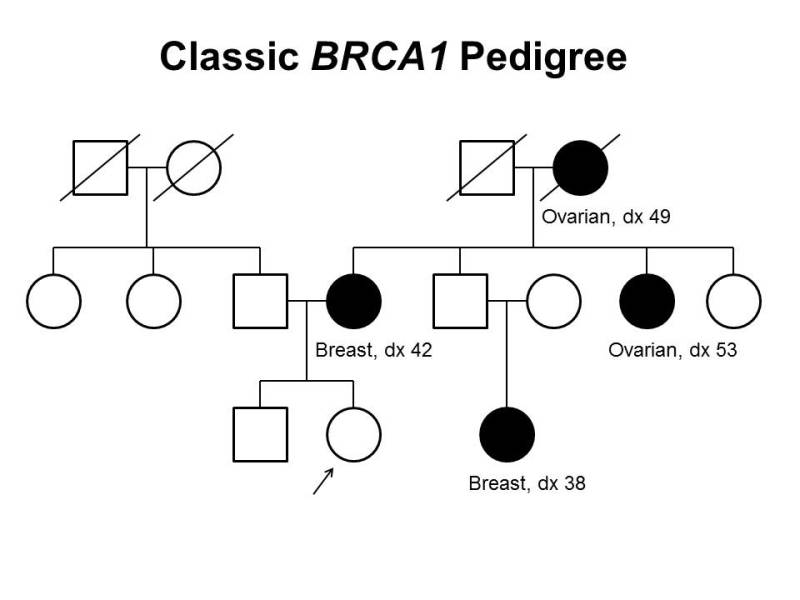
\includegraphics{ACMG-figure/pedigree.jpg}

\end{frame}

\begin{frame}{Segregation data (BS1, PP1)}
\protect\hypertarget{segregation-data-bs1-pp1}{}

\begin{itemize}
\tightlist
\item
  Caveat: linkage disequilibrium\\
\item
  Penetration rate\\
\item
  Difficult statistical evaluation
\end{itemize}

\end{frame}

\begin{frame}{Population data}
\protect\hypertarget{population-data}{}

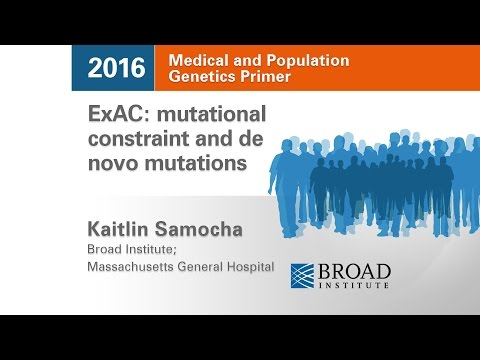
\includegraphics{ACMG-figure/gnomad.jpg}

\end{frame}

\begin{frame}{Population data}
\protect\hypertarget{population-data-1}{}

\begin{itemize}
\tightlist
\item
  To high minor allele frequency (MAF)
\item
  5\%: benign stand alone (BA1)\\
\item
  1\% ?? (Think about prevalence of HBOCS) (BS1)\\
\item
  Wow! The first time observed variant! (Absent in population DB, PM2)
\end{itemize}

\end{frame}

\begin{frame}{Null variant}
\protect\hypertarget{null-variant}{}

\begin{itemize}
\tightlist
\item
  Frameshift, Nonsense, canonical +-1 or 2 splicing site, initiation
  codon
\item
  Caveat: LOF variants at the extreme 3′ end of a gene\\
\item
  Caveat: presence of multiple transcripts
\end{itemize}

\end{frame}

\begin{frame}{Computational (in silico) data}
\protect\hypertarget{computational-in-silico-data}{}

\begin{itemize}
\tightlist
\item
  PolyPhen2, SIFT, MutationTaster, etc\\
\item
  Mutational hot spot and/or critical and wellestablished (PM1)\\
\item
  Protein length changes due to in-frame deletions/insertions and stop
  losses functional domain (PM4 BP3)\\
\item
  Novel missense at the same position (PM5)
\end{itemize}

\end{frame}

\begin{frame}{Other evidence}
\protect\hypertarget{other-evidence}{}

\begin{itemize}
\tightlist
\item
  de novo variants (PS2 PM6)
\item
  functional studies (PS3 BS3)
\item
  Computational (in silico) data\\
\item
  Allelic data (BP2 PM3)\\
\item
  Phenotype to support variant claims
\end{itemize}

\end{frame}

\begin{frame}{Evidences of interpretation}
\protect\hypertarget{evidences-of-interpretation}{}

\begin{itemize}
\tightlist
\item
  Population data\\
\item
  Computational data\\
\item
  Functional data\\
\item
  Segregation data\\
\item
  De novo data\\
\item
  Allele data\\
\item
  Other databases\\
\item
  Other data
\end{itemize}

\end{frame}

\begin{frame}{ACMG Standards and guidelines for interpretation of
sequence variants}
\protect\hypertarget{acmg-standards-and-guidelines-for-interpretation-of-sequence-variants}{}

\includegraphics{https://media.nature.com/lw926/nature-assets/gim/journal/v17/n5/images/gim201530f1.jpeg}

\end{frame}

\begin{frame}{Rules for combining criteria to classify sequence
variants}
\protect\hypertarget{rules-for-combining-criteria-to-classify-sequence-variants}{}

\includegraphics{https://media.nature.com/full/nature-assets/gim/journal/v17/n5/images/gim201530t5.jpeg}

\end{frame}

\begin{frame}{Which evidences are available in our lab?}
\protect\hypertarget{which-evidences-are-available-in-our-lab}{}

\end{frame}

\begin{frame}{Population, disease-specific, and sequence databases}
\protect\hypertarget{population-disease-specific-and-sequence-databases}{}

\includegraphics{https://media.nature.com/full/nature-assets/gim/journal/v17/n5/images/gim201530t1.jpeg}

\end{frame}

\begin{frame}{In silico predictive algorithms}
\protect\hypertarget{in-silico-predictive-algorithms}{}

\includegraphics{https://media.nature.com/full/nature-assets/gim/journal/v17/n5/images/gim201530t2.jpeg}

\end{frame}

\begin{frame}{Criteria for classifying pathogenic variants}
\protect\hypertarget{criteria-for-classifying-pathogenic-variants}{}

\includegraphics{https://media.nature.com/full/nature-assets/gim/journal/v17/n5/images/gim201530t3.jpeg}

\end{frame}

\begin{frame}{Criteria for classifying benign variants}
\protect\hypertarget{criteria-for-classifying-benign-variants}{}

\includegraphics{https://media.nature.com/full/nature-assets/gim/journal/v17/n5/images/gim201530t4.jpeg}

\end{frame}

\begin{frame}{Example}
\protect\hypertarget{example}{}

\begin{itemize}
\tightlist
\item
  Temporal bone abnormalities detected by computed tomography in a
  hearing-impaired patient
\item
  Uncertain variant in SLC26A4, the gene associated with Pendred
  syndrome
\item
  Testing other family members to establish when a variant is \textbf{de
  novo}
\item
  Variant \textbf{cosegregates} with disease in the family
\item
  Variant is in \textbf{trans with a pathogenic variant} in the same
  recessive disease-causing gene
\item
  Filtering out or discounting the vast majority of variants for
  dominant diseases when they can be observed in healthy relatives is
  possible
\end{itemize}

Making the interpretation much more efficient and conclusive

\end{frame}

\begin{frame}{CMC pathology lab}
\protect\hypertarget{cmc-pathology-lab}{}

\begin{itemize}
\tightlist
\item
  In house database\\
\item
  \url{https://brcaexchange.org/variants?search=p.Arg3384Ter}
\item
  \url{http://152.99.75.168/KRGDB/}~\\
\item
  \url{https://www.ncbi.nlm.nih.gov/clinvar/variation/51049/}~\\
\item
  \url{https://gnomad.broadinstitute.org/variant/13-32972800-C-T}
\end{itemize}

\end{frame}

\begin{frame}{KOBRA\textsuperscript{2}}
\protect\hypertarget{kobra--kang_2015_prevalence_breastcancerrestreat}{}

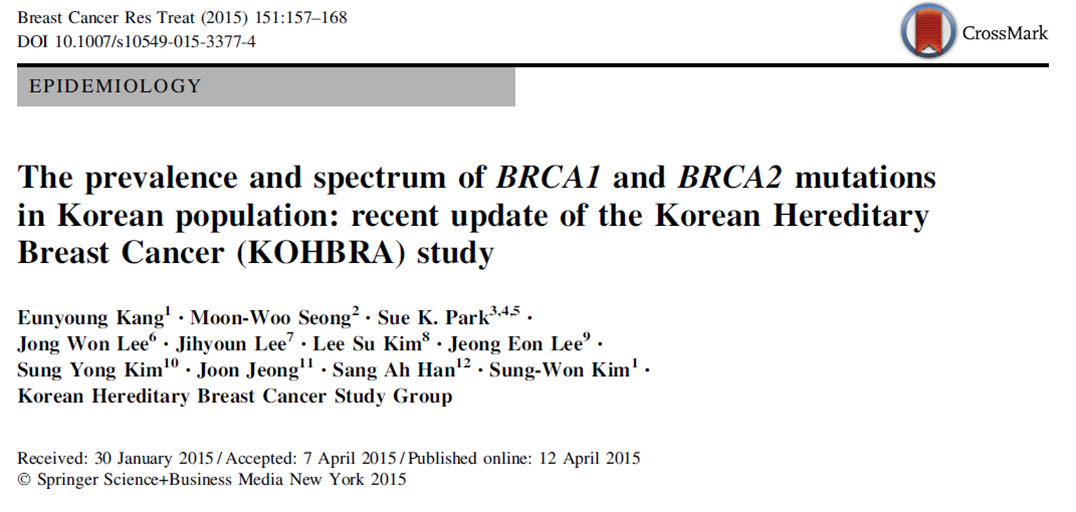
\includegraphics{KOBRA_head.png} 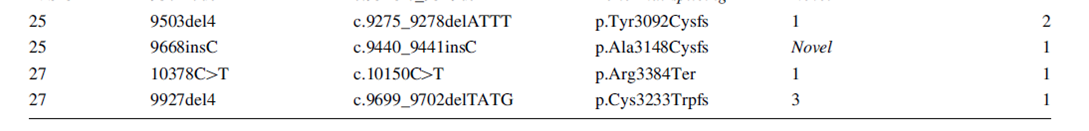
\includegraphics{KOBRA.png}

\end{frame}

\begin{frame}{End truncation}
\protect\hypertarget{end-truncation}{}

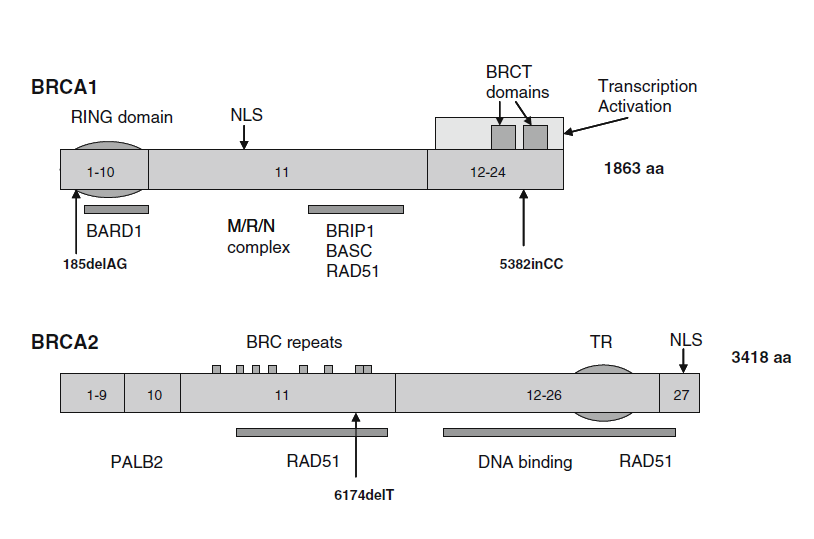
\includegraphics{BRCA2.png}

\end{frame}

\begin{frame}{HUMAN MUTATION Mutation in Brief 31: E 1200-E1240 (2010)
Online}
\protect\hypertarget{human-mutation-mutation-in-brief-31-e-1200-e1240-2010-online}{}

Finally, three sequence variants -- BRCA2 c.9976A\textgreater{}T (BIC:
K3326X), c.10095delCins11 (BIC: 10323delCins11) and
c.10150C\textgreater{}T (BIC: \textbf{R3384X}) predicted to result in
protein truncation were ruled as exceptions that \textbf{could not be
classified} because of their \textbf{location near the 3´-end} and
possibly dispensable part of the gene.

\end{frame}

\begin{frame}{Conclusions}
\protect\hypertarget{conclusions}{}

\begin{itemize}
\tightlist
\item
  Interpretaion of sequence variants
\item
  Knowledge base (ClinVar, BRCAexchange \ldots{})
\item
  VUS
\end{itemize}

\end{frame}

\begin{frame}{Allele frequency in Somatic vs Germline in tumor only
sample}
\protect\hypertarget{allele-frequency-in-somatic-vs-germline-in-tumor-only-sample}{}

\begin{itemize}
\tightlist
\item
  BRCA1 mutation: Positive - p.Glu649Ter (c.1945G\textgreater{}T)\\
\item
  Variant allele frequency 63.84\%\\
\item
  Tumor cell percentage: 70\%
\end{itemize}

\end{frame}

\begin{frame}{Allele frequency in Somatic vs Germline in tumor only
sample\textsuperscript{3}}
\protect\hypertarget{allele-frequency-in-somatic-vs-germline-in-tumor-only-sample-sun_2018_computational_ploscomputationalbiology}{}

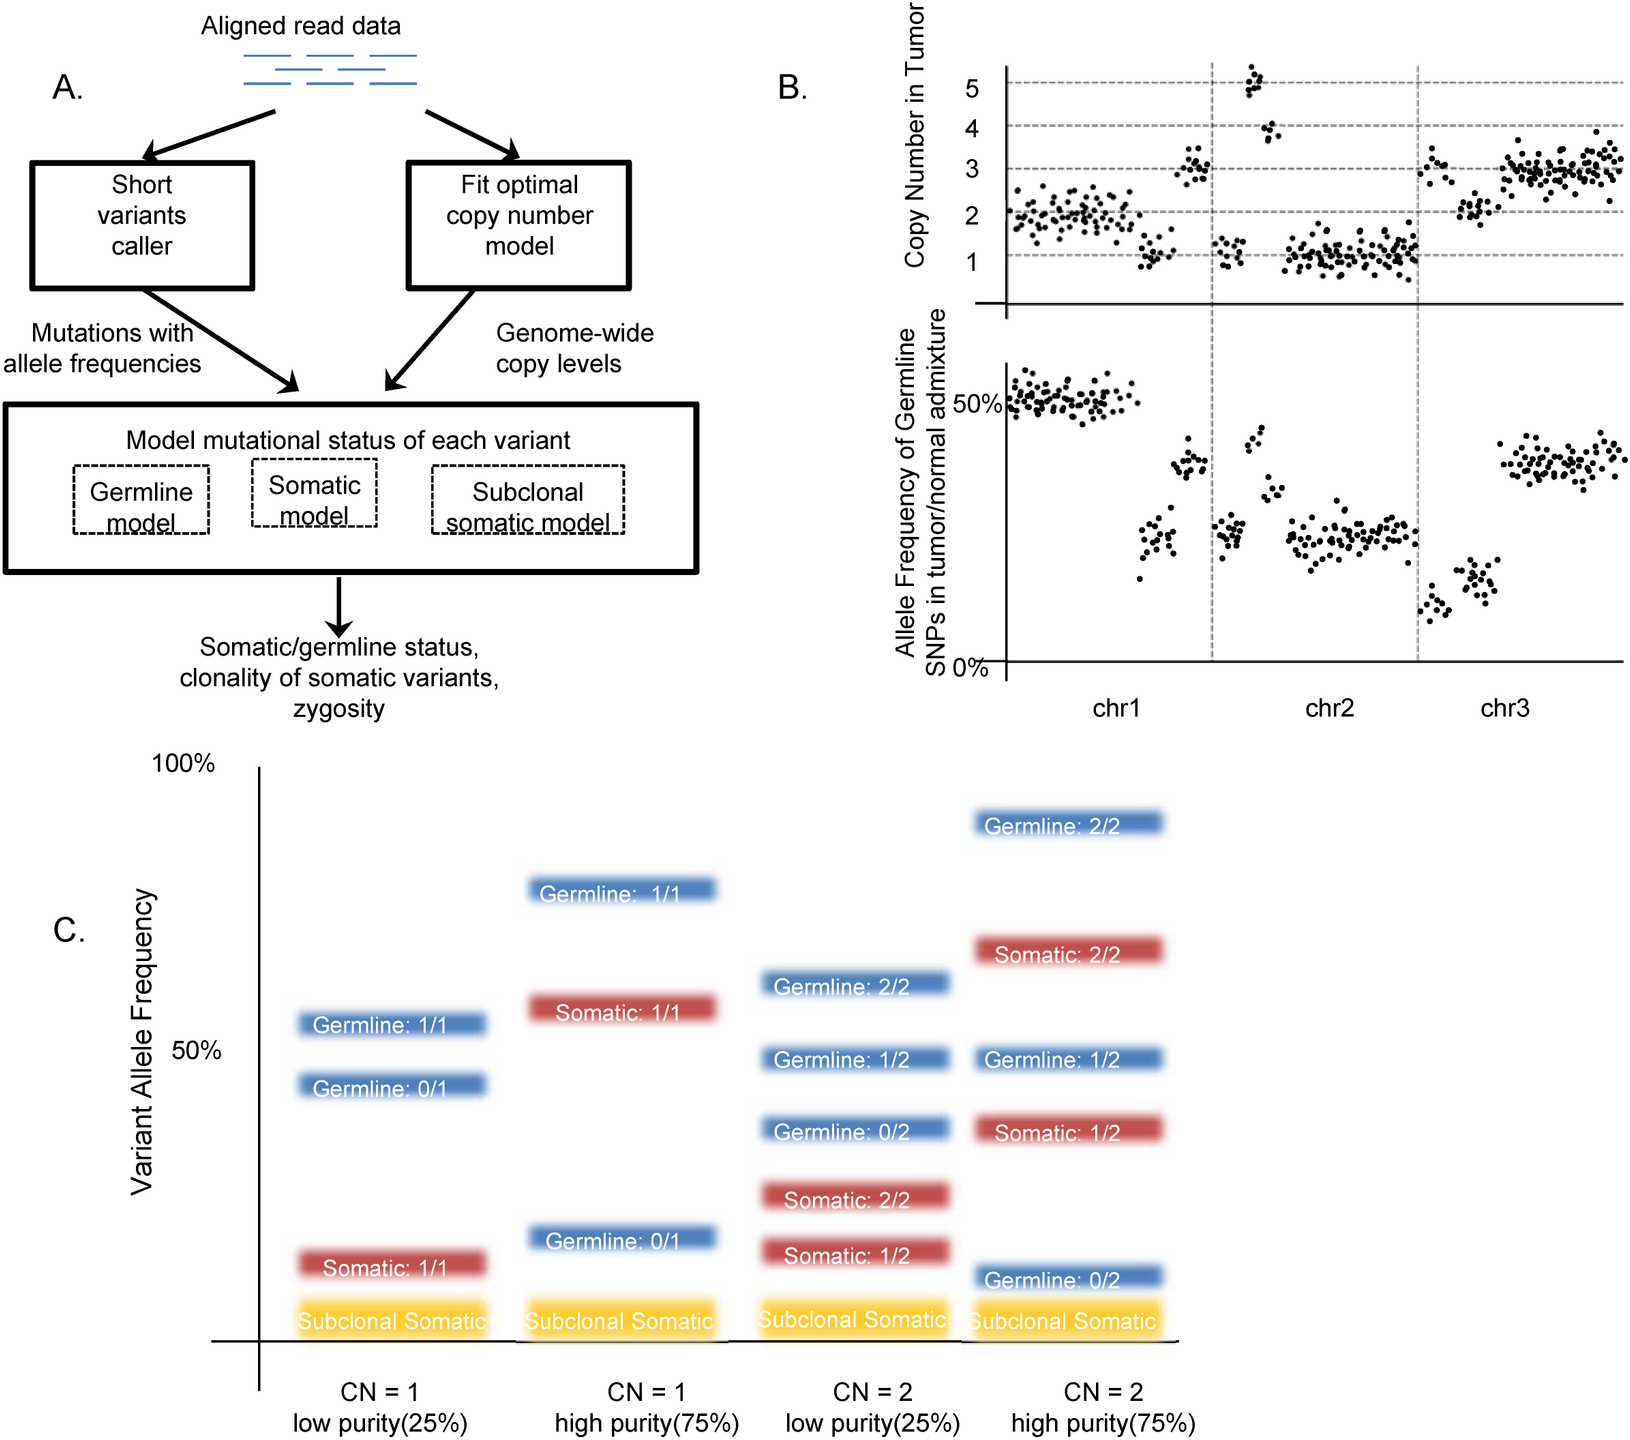
\includegraphics{https://journals.plos.org/ploscompbiol/article/figure/image?size=large\&id=10.1371/journal.pcbi.1005965.g001}

\end{frame}

\begin{frame}{Allele frequency in Somatic vs Germline in tumor only
sample\textsuperscript{3}}
\protect\hypertarget{allele-frequency-in-somatic-vs-germline-in-tumor-only-sample-sun_2018_computational_ploscomputationalbiology-1}{}

\begin{itemize}
\tightlist
\item
  BRCA1 mutation: Positive - p.Glu649Ter (c.1945G\textgreater{}T)\\
\item
  Variant allele frequency 63.84\%\\
\item
  Tumor cell percentage: 70\%
\end{itemize}

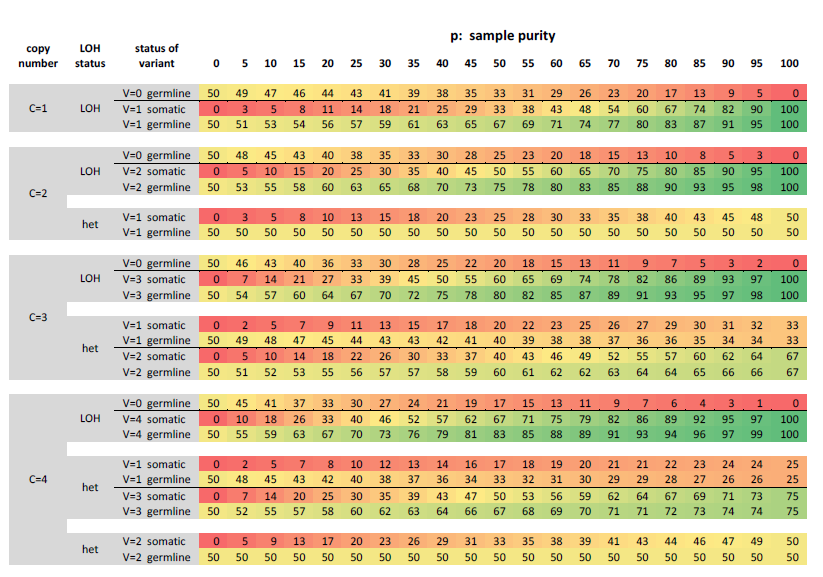
\includegraphics{https://www.jkangpathology.com/img/AF.png}
\url{https://journals.plos.org/ploscompbiol/article/file?id=10.1371/journal.pcbi.1005965.s003\&type=supplementary}

\end{frame}

\begin{frame}{References}
\protect\hypertarget{references}{}

\hypertarget{refs}{}
\leavevmode\hypertarget{ref-richards_2015_standards_genetmeda}{}%
1. Richards, S., Aziz, N., Bale, S., Bick, D., Das, S., Gastier-Foster,
J., Grody, W.W., Hegde, M., Lyon, E., Spector, E., et al. (2015).
Standards and guidelines for the interpretation of sequence variants: A
joint consensus recommendation of the American College of Medical
Genetics and Genomics and the Association for Molecular Pathology.
Genetics in Medicine \emph{17}, 405--423.

\leavevmode\hypertarget{ref-kang_2015_prevalence_breastcancerrestreat}{}%
2. Kang, E., Seong, M.-W., Park, S.K., Lee, J.W., Lee, J., Kim, L.S.,
Lee, J.E., Kim, S.Y., Jeong, J., Han, S.A., et al. (2015). The
prevalence and spectrum of BRCA1 and BRCA2 mutations in Korean
population: Recent update of the Korean Hereditary Breast Cancer
(KOHBRA) study. Breast Cancer Res Treat \emph{151}, 157--168.

\leavevmode\hypertarget{ref-sun_2018_computational_ploscomputationalbiology}{}%
3. Sun, J.X., He, Y., Sanford, E., Montesion, M., Frampton, G.M.,
Vignot, S., Soria, J.-C., Ross, J.S., Miller, V.A., Stephens, P.J., et
al. (2018). A computational approach to distinguish somatic vs. Germline
origin of genomic alterations from deep sequencing of cancer specimens
without a matched normal. PLOS Computational Biology \emph{14},
e1005965.

\end{frame}

\end{document}
